
\subsection{Classi Principali}

In figura~\ref{fig:classi-principali} sono illustrati i package e le classi principali del sistema di HBS, come definite sopra.
Lo stereotipo \code{<<Intercepted>>} identifica classi i cui metodi sono intercettati dal sistema di logging (v.\ sotto).

\begin{figure*}[h]
    \centering
    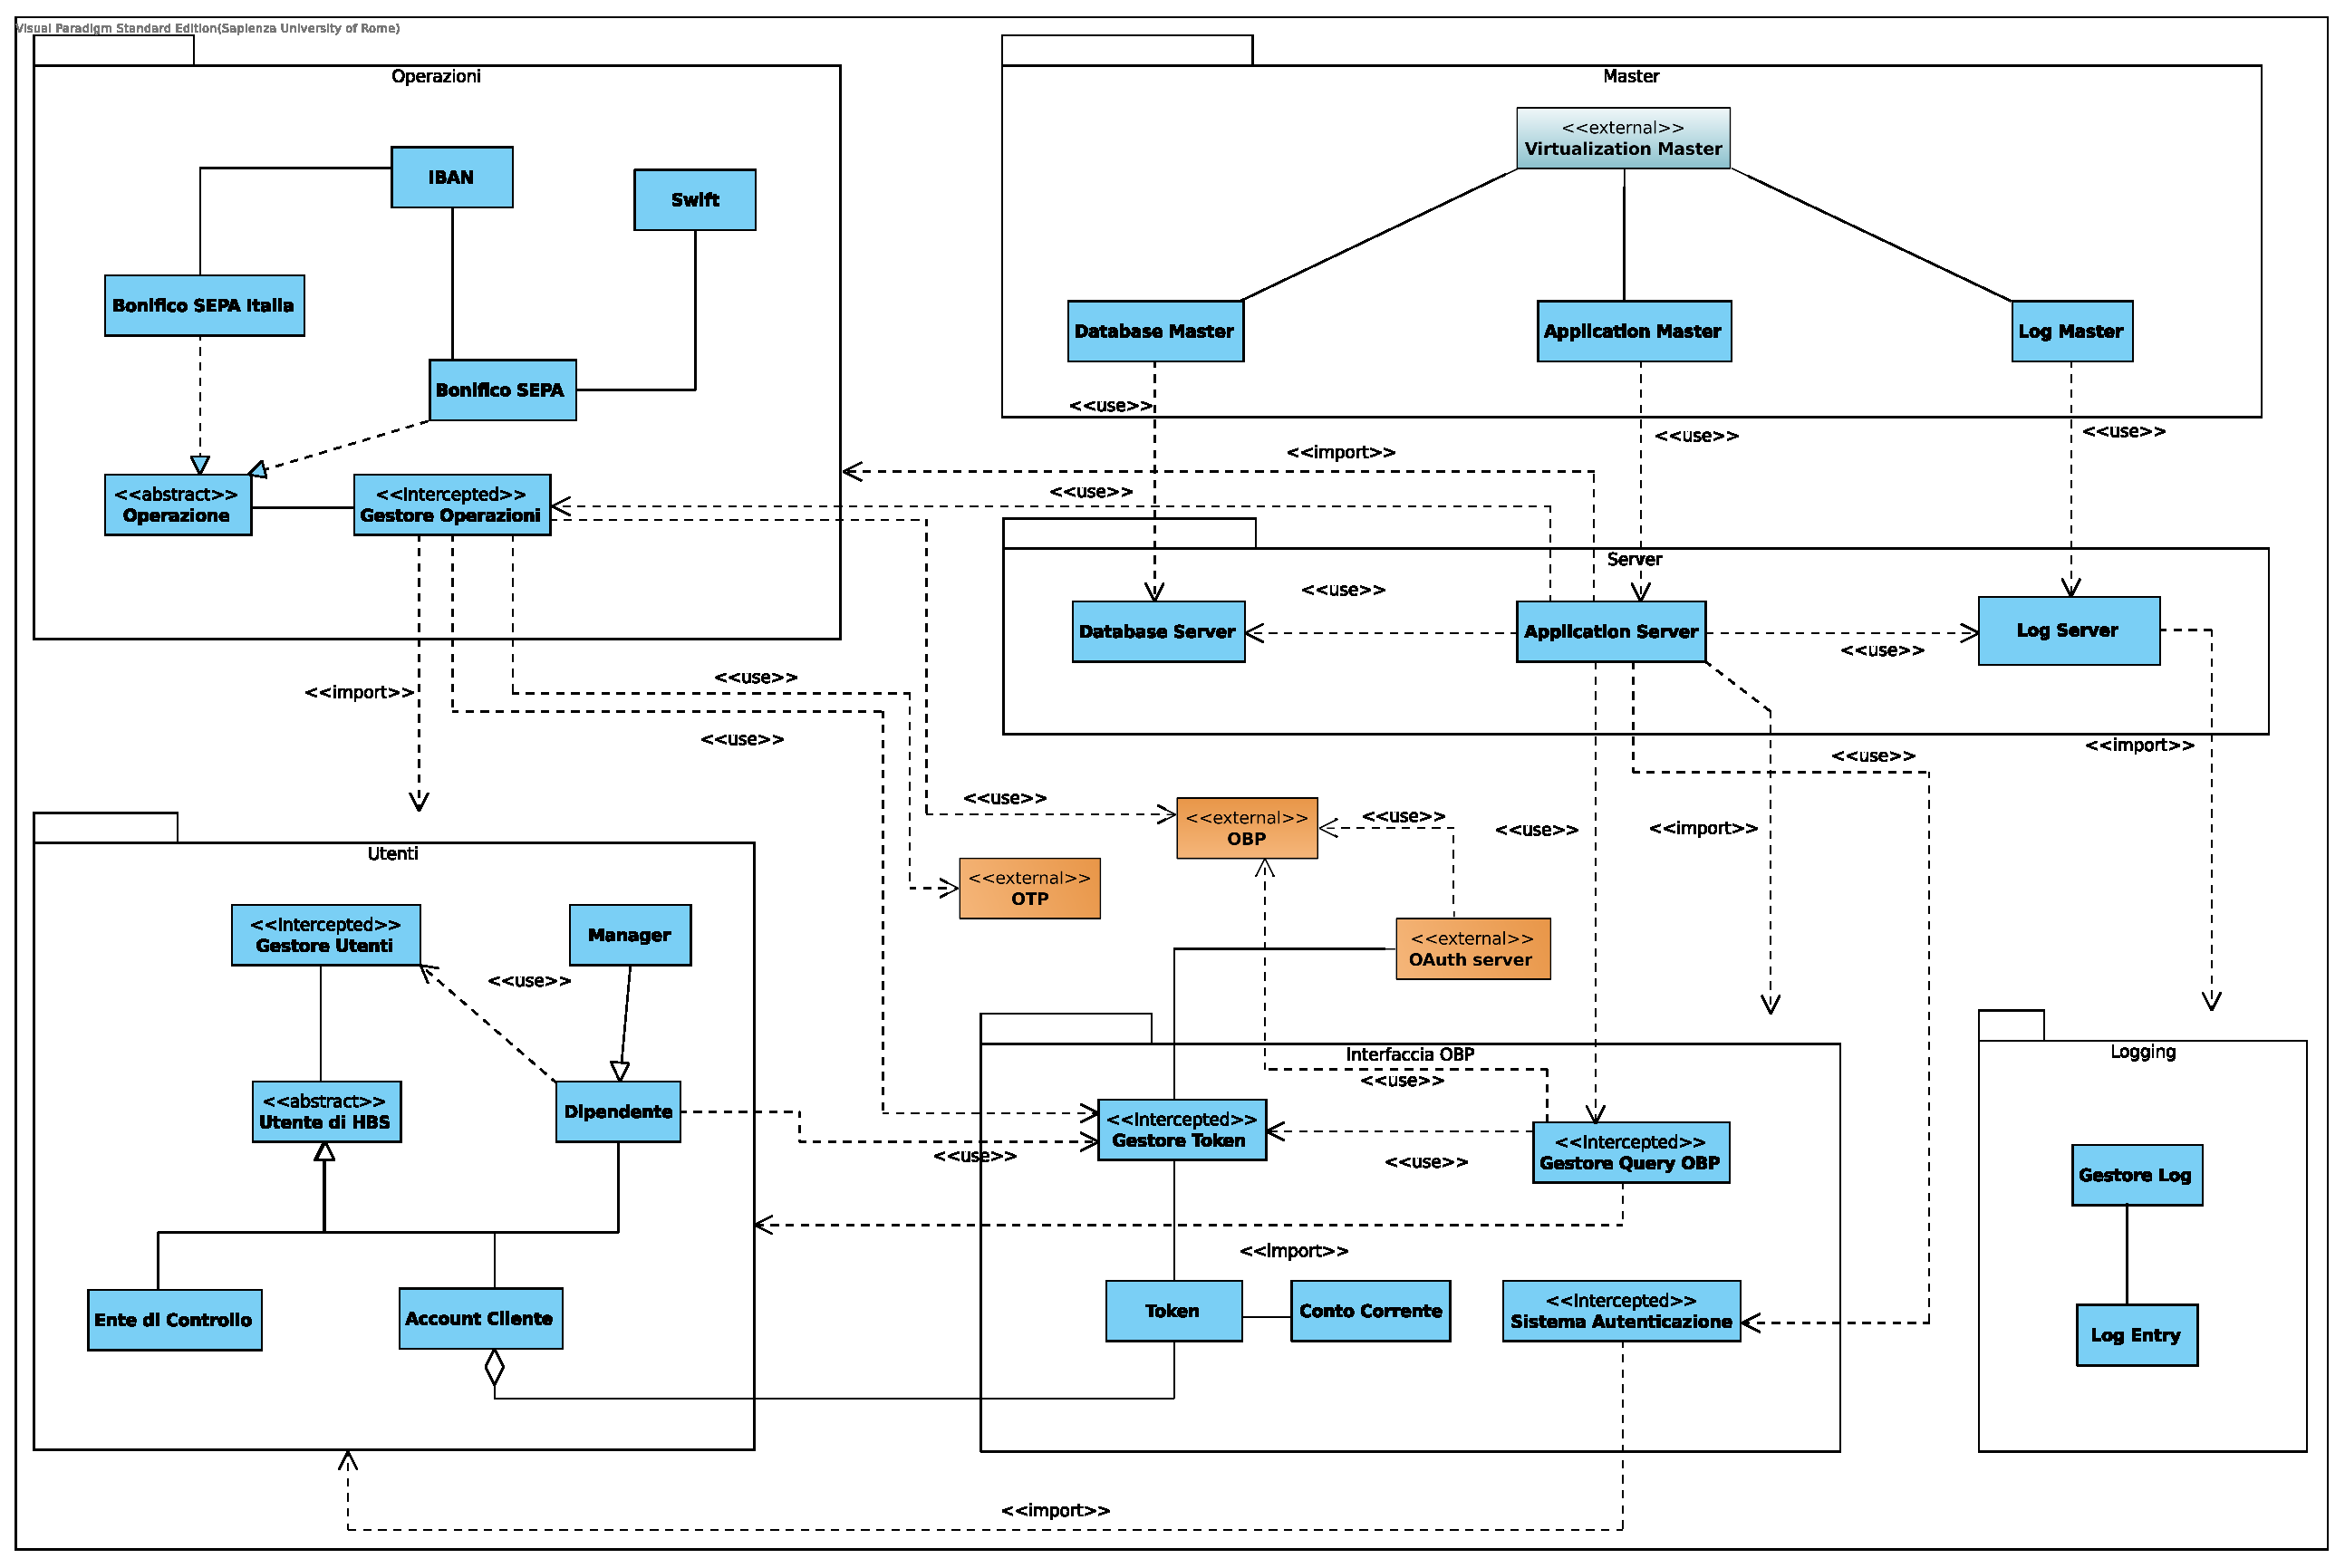
\includegraphics[width=\textheight, angle=90]{Images/Classi_Design.eps}
    \caption{Diagramma delle classi di design di HBS, ristretto alle classi principali.}
    \label{fig:classi-principali}
\end{figure*}

In figura~\ref{fig:classi-principali:operazioni} sono illustrate nel dettaglio le classi del package relativo alle operazioni.

\begin{figure*}[h]
    \centering
    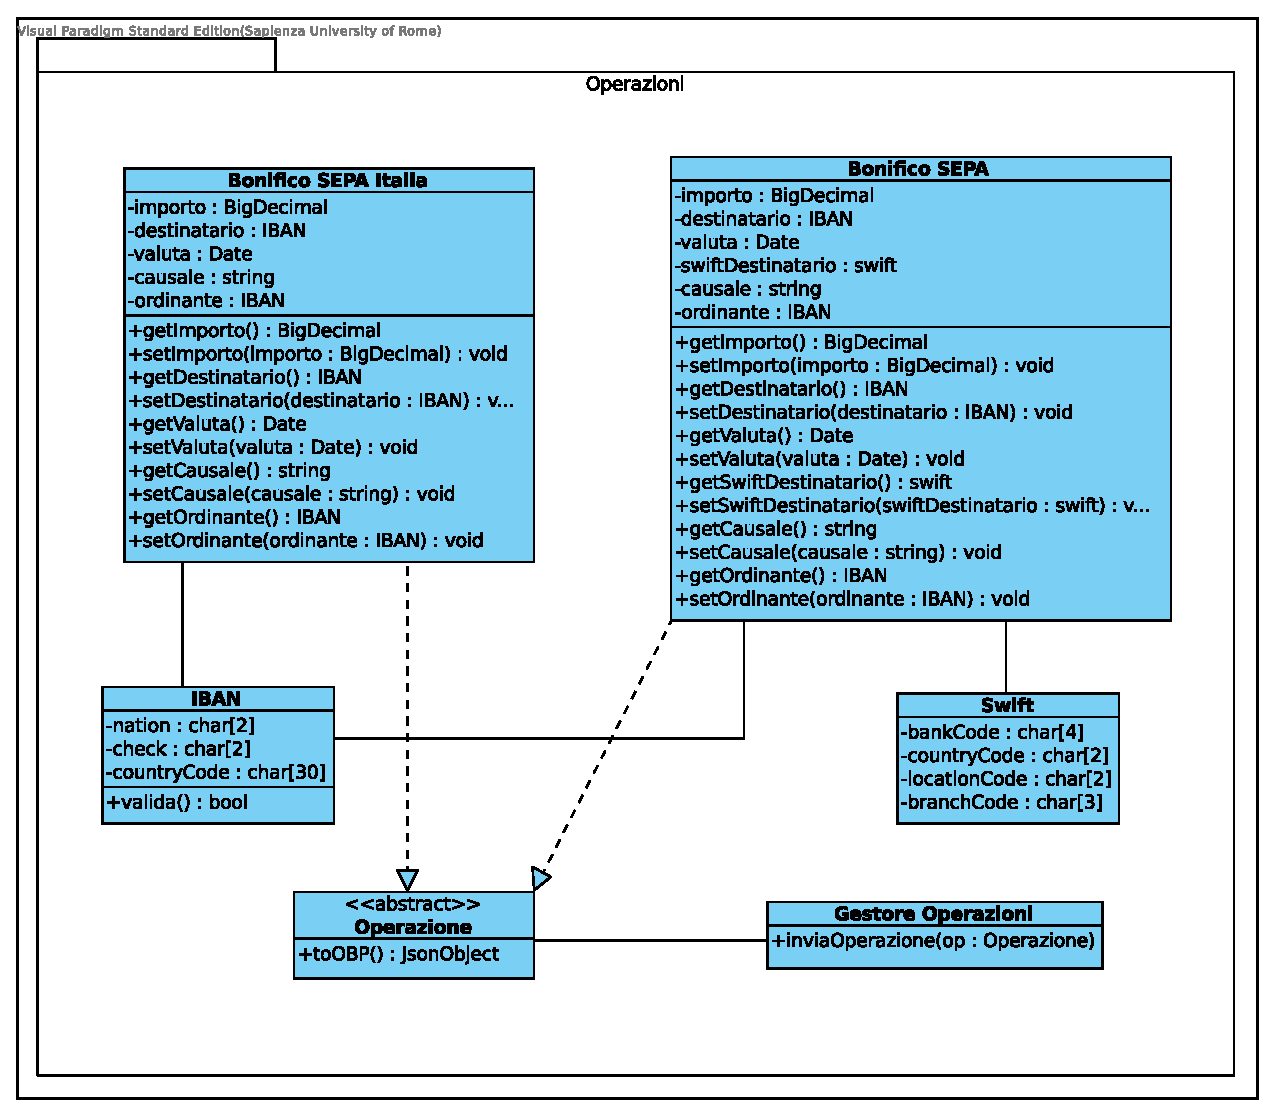
\includegraphics[width=\textwidth]{Images/Operazioni_Design.eps}
    \caption{Diagramma delle classi relative alle operazioni del sistema HBS.}
    \label{fig:classi-principali:operazioni}
\end{figure*}

In figura~\ref{fig:classi-principali:log} sono illustrate le classi del package relativo al sistema di logging.
Il sotto-sistema di logging utilizza il sistema di \emph{Class Interceptors} presente in Java EE 7.
Le annotazioni dei metodi sono riportate in figura come stereotipi.
Lo stereotipo \code{<<AroundInvoke>>} identifica l'annotazione \code{@AroundInvoke}.

I metodi delle classi soggette a logging sono decorati dallo stereotipo \code{Intercepted}, a cui corrisponde l'annotazione \code{@Interceptors(GestoreLog.class)}.
Le classi soggette a logging sono:
\begin{itemize}
	\item Gestore Operazioni;
	\item Gestore Query OBP;
	\item Gestore Token;
	\item Sistema Autenticazione.
\end{itemize}

\begin{figure*}[h]
    \centering
    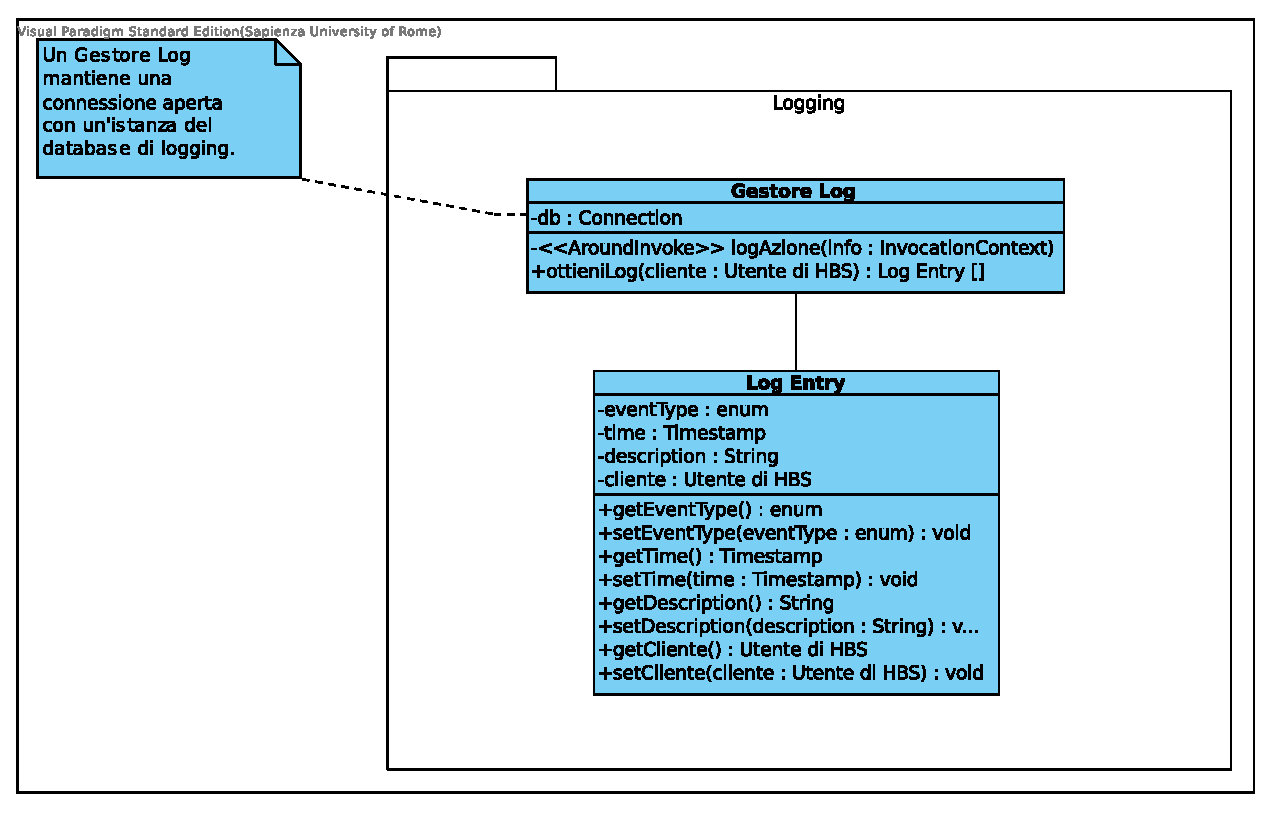
\includegraphics[width=\textwidth]{Images/Logging.eps}
    \caption{Diagramma delle classi relative al sotto-sistema di Logging.}
    \label{fig:classi-principali:log}
\end{figure*}

